\documentclass[letterpaper, 10 pt, conference]{IEEEtran}  % Comment this line out if you need a4paper

%\documentclass[a4paper, 10pt, conference]{ieeeconf}      % Use this line for a4 paper

\IEEEoverridecommandlockouts                              % This command is only needed if 
% you want to use the \thanks command

%\overrideIEEEmargins                                      % Needed to meet printer requirements.

\usepackage{amsmath, amssymb}
\usepackage{amsfonts}

\let\yesnumberold=\yesnumber\relax
\let\yesnumber\relax
\usepackage[math]{easyeqn}
\let\yesnumber\yesnumberold

\usepackage{bm}
\usepackage{multirow}
\usepackage{graphicx}
\setcounter{MaxMatrixCols}{30}
\usepackage{epstopdf}
\usepackage{enumerate}
\usepackage{color}

\usepackage{booktabs, tabularx}
\usepackage{multirow}

\usepackage{epstopdf}
\usepackage{epsfig}
\usepackage{subfigure}

\usepackage{algorithm}
\usepackage{algpseudocode}


\include{include/math_commands}

\usepackage{hyperref}

% Label definitions

% Vectors
\def\x{{\mathbf x}}

% Sets
\def\R{\mathbb{R}}
\def\N{\mathbb{N}}
\def\Z{\mathbb{Z}}

% Stochastic
\def\Pr#1{\ensuremath{\text{Pr}\left [#1 \right ]}}
\def\E#1{\ensuremath{\text{E}\left \{#1 \right \}}}

% Matrix measures
\newcommand{\tr}[1]{{\mbox{Trace}\left (#1\right) }}

% CBS
\newcommand{\cbs}{\textsf{CBS}}

% Math operations
\newcommand{\ceil}[1]{\left\lceil #1 \right\rceil}
\newcommand{\floor}[1]{\left\lfloor #1 \right\rfloor}

\DeclareMathOperator*{\argmax}{arg\,max}
\DeclareMathOperator{\softmax}{softmax}

% Frames
\newcommand{\frm}[1]{\langle #1\rangle}

% Theorems
\newtheorem{theorem}{Theorem}
\newtheorem{acknowledgement}[theorem]{Acknowledgement}
%\newtheorem{algorithm}[theorem]{Algorithm}
\newtheorem{axiom}[theorem]{Axiom}
\newtheorem{case}[theorem]{Case}
\newtheorem{claim}[theorem]{Claim}
\newtheorem{conclusion}[theorem]{Conclusion}
\newtheorem{condition}[theorem]{Condition}
\newtheorem{conjecture}[theorem]{Conjecture}
\newtheorem{corollary}[theorem]{Corollary}
\newtheorem{criterion}[theorem]{Criterion}
\newtheorem{definition}[theorem]{Definition}
\newtheorem{example}[theorem]{Example}
\newtheorem{exercise}[theorem]{Exercise}
\newtheorem{lemma}[theorem]{Lemma}
\newtheorem{notation}[theorem]{Notation}
\newtheorem{problem}[theorem]{Problem}
\newtheorem{proposition}{Proposition}
\newtheorem{remark}{Remark}
\newtheorem{solution}[theorem]{Solution}
\newtheorem{summary}[theorem]{Summary}
\newtheorem{assumption}[theorem]{Assumption}
\newtheorem{property}[theorem]{Property}

% Comments
\newcommand{\lui}[1]{\color{green}{{\bf #1}}\color{black}}
\newcommand{\dan}[1]{\color{red}{{\bf #1}}\color{black}}
\newcommand{\ale}[1]{\textcolor{blue}{\bf #1}}
\newcommand{\pla}[1]{\textcolor{cyan}{\bf #1}}
\newcommand{\rev}[1]{\color{blue}{{#1}}\color{black}}

% Cartesian product
\global\long\def\cart{\operatorname*{\diagup\hspace{-9pt}\diagdown}}

% Text rotation
\newcommand\RotText[1]{\rotatebox{90}{\parbox{3.5cm}{\centering#1}}}

\title{\LARGE \bf Climbing robot}

\author{Marco Frego, MIchele Focchi, 
	Luigi Palopoli, .....
	%Alessandro Antonucci$^{1}$, Placido Falqueto$^{1}$,
	%	Luigi Palopoli$^{1}$, Daniele Fontanelli$^{2}$ %\vspace{0.1cm}
	%\IEEEoverridecommandlockouts
	% \IEEEpubid{\makebox[\columnwidth]
		% 	{\hfill : 978-1-5090-6299-7/17/\$31.00~\copyright~2017 European Union}
		%	\hspace{\columnsep}\makebox[\columnwidth]{ }}
	%\thanks{$^{1}$A. Antonucci,	P. Falqueto, and L. Palopoli
		%    are with the Department of Information Engineering and Computer Science (DISI), University of Trento, Via Sommarive 9, Trento, Italy (e-mail:
		%		\{alessandro.antonucci, placido.falqueto, luigi.palopoli\}@unitn.it) }%
	%\thanks{$^{2}$D. Fontanelli is with the Department
		%	of Industrial Engineering (DII), University of Trento, Via
		%	Sommarive 9, Trento, Italy (e-mail:
		%	daniele.fontanelli@unitn.it) }
}

\begin{document}
	
	\maketitle
	\thispagestyle{empty}
	\pagestyle{empty}
	
	
	
	\begin{abstract}
		
	\end{abstract}
	
	%%%%%%%%%%%%%%%%%%%%%%%%%%%%%%%%%%%%%%%%%%%%%%%%%%%%%%%%%%%%%%%%%%%%%%%%%%%%%%%%
	
	\section{Model}
	The spherical pendulum model is shown in figure \ref{fig:sp} . where $\theta$ is the polar angle [rad] and $\phi$ is the Azimuth angle [rad] . \\ 
	\begin{figure}
		\includegraphics[width=\columnwidth]{figs/spherical_pendulum}
		\caption{Spherical pendulum}
		\label{fig:sp}
	\end{figure}
	We assume that:
	\begin{enumerate}
		\item The friction can be neglected
		\item The mass is entirely concentrated in the body attached to the wire
		\item The wire can be unwounded and rewounded but it is rigid and remains completely elongated (i.e., it cannot make bends)
		\item The rewinder can pull the wire when winding it but cannot push it (i.e., it can only act as a brake during the unwinding phase)
		\item The system is acted on by the following forces:
		\begin{itemize}
			\item The mass weight
			\item The rewinder pull action or braking action $\mathbf{F}_r$ oriented along the wire
			\item An impulsive push force $\mathbf{F}_u$ that the robot can generate when it is attached to the mountain wall
		\end{itemize}
	\end{enumerate}
	Let $e$ be a frame attached to the mass and with axis oriented along the $x$ axis and let $w$ be the world frame attached to
	the suspension point of the pendulum.
	If we consider the homogeneous transformation linking $e$ to $w$, we can write:
	\[
	T_e^w = \begin{bmatrix} R_z(\phi) &\begin{matrix}0\\0\\0 \end{matrix}  \\ \begin{matrix} 0 &0 &0 \end{matrix} & 1\end{bmatrix}  \begin{bmatrix} R_y(\pi/2 - \theta) &\begin{matrix}0\\0\\0 \end{matrix}  \\ \begin{matrix} 0 &0 &0 \end{matrix} & 1\end{bmatrix}  \begin{bmatrix} I_{3,3} &\begin{matrix}0\\0\\0 \end{matrix}  \\ \begin{matrix} L &0 &0 \end{matrix} & 1\end{bmatrix}  
	\]
	where $R_z(\phi)$ is the rotation matrix of $\phi$ around $z$ and $R_y(\alpha)$ is the rotation matrix of $\alpha$ around $y$.
	Overall, we have:
	\[
	T_e^w = \begin{bmatrix} c_\phi s_\theta & -s_\phi & c_\phi c_\theta & l c_\phi s_\theta\\
		s_\phi s_\theta & c_\phi & c_\theta s_\phi & l s_\phi s_\theta\\
		-c_\theta & 0 & s_\theta &-l c_\theta\\
		0 & 0 &0 &1\end{bmatrix}
	\]
	where $c_x$ is a shorthand for $\cos x$ and $s_x$ is a shorthand for $\sin x$.
	From this equation, we have that the position $\mathbf{p}$ of the mass is given by:
	\begin{align} \label{eq1}
		\mathbf{p} = \begin{bmatrix} x\\ y\\ z \end{bmatrix} =
		\begin{bmatrix} l s_\theta c_\phi\\
			l s_\theta s_\phi\\
			-l c_\theta \end{bmatrix}
	\end{align}
	From equation \ref{eq1}, the velocities along the axes are:  
	\begin{align*}
		\dot{x} &= 
		l c_\theta c_\phi \dot{\theta} - l s_\theta s_\phi \dot{\phi} + s_\theta c_\phi \dot{l} \\
		\dot{y} &= l c_\theta s_\phi \dot{\theta} + l s_\theta c_\phi \dot{\phi} + s_\theta s_\phi \dot{l} \\
		\dot{z} &= l s_\theta  \dot{\theta} - c_\theta \dot{l} 
	\end{align*}
Next, the velocity of the mass is :
	\begin{align*}
		v^2 &= \dot{x}^2 + \dot{y}^2 + \dot{z}^2 \\		
		&=  l^2 c_\theta^2 c_\phi^2 \dot{\theta}^2 + l^2 s_\theta^2 s_\phi^2 \dot{\phi}^2 + s_\theta^2 c_\phi^2 \dot{l}^2 - 2l^2 c_\theta s_\theta c_\phi s_\phi   \dot{\theta} \dot{\phi} - 2l s_\theta^2 s_\phi c_\phi \dot{l} \dot{\phi} \\
		& + 2l c_\theta s_\theta c_\phi^2  \dot{\theta} \dot{l} + l^2 c_\theta^2 s_\phi^2 \dot{\theta}^2 + l^2 s_\theta^2 c_\phi^2 \dot{\phi}^2 + s_\theta^2 s_\phi^2 \dot{l}^2 + 2l^2 c_\theta s_\theta s_\phi c_\phi \dot{\theta} \dot{\phi} \\
		&+ 2l s_\theta^2 c_\phi s_\phi \dot{l} \dot{\phi} + 2l c_\theta s_\theta s_\phi^2  \dot{\theta} \dot{l} + l^2 s_\theta^2  \dot{\theta}^2 + c_\theta^2 \dot{l}^2 - 2l s_\theta c_\theta   \dot{\theta} \dot{l} \\ \\
		&= l^2 c_\theta^2 \left(c_\phi^2 + s_\phi^2\right) \dot{\theta}^2 + l^2 s_\theta^2  \left( s_\phi^2 + c_\phi^2 \right) \dot{\phi}^2 + l^2 s_\theta^2  \dot{\theta}^2 + \dot{l}^2 s_\theta^2 \left(c_\phi^2 + s_\phi^2\right) \\
		&+ 2l c_\theta s_\theta \left(c_\phi^2 + s_\phi^2\right) \dot{\theta} \dot{l} + c_\theta^2 \dot{l}^2 - 2l s_\theta c_\theta \dot{\theta} \dot{l} \\  \\
		&=  l^2 \dot{\theta}^2 + l^2 s_\theta^2 \dot{\phi}^2 + \dot{l}^2\\
	\end{align*}
	
	Thus, the kinetic energy $T$ of the system :
	\begin{align*}
		T &=\frac{ m }{2} v^2 \\
		&= \frac{m}{2} \left(\dot{x}^2 + \dot{y}^2 + \dot{z}^2\right) \\
		&=  \frac{m}{2} l^2 \left(\dot{\theta}^2 + s_\theta^2 \dot{\phi}^2 \right) + \frac{m }{2} \dot{l}^2 \\
	\end{align*}
And the potential energy $V$ :
		\begin{align*}
		V &= mgz\\
		&= -mgl c_\theta
	\end{align*}
 The Lagrangian function is given by:
	\begin{equation}
		L = T - V = \frac{m}{2} l^2 \left(\dot{\theta}^2 + s_\theta^2 \dot{\phi}^2\right) + \frac{m}{2}\dot{l}^2 + mgl c_\theta
	\end{equation}
	The generalized coordinates are in this case given by $q_1 = \theta, q_2 = \phi,$ and $q_3 = l$ .
	If we apply the d'Alembert principle, the Lagrangian Equation can be written as:
	\[
	\frac{d}{dt}\frac{\partial L}{\partial \dot{q}_i} - \frac{\partial L}{\partial q_i} = Q_i^p ,
	\]
	where $Q_i^p$ is the generalized force $Q_i^p = (\mathbf{F}_r + \mathbf{F}_u) \cdot \frac{\partial \mathbf{p}}{\partial q_i}$.
	Observe that  $\mathbf{F}_r$ oriented along the rope and $\mathbf{F}_u$ does not have any component along the rope (otherwise
	it will forms bends):
	\begin{align*}
		\mathbf{F}_r  &= F_r \begin{bmatrix}
			c_\phi s_\theta\\
			s_\phi s_\theta\\
			-c_\theta
		\end{bmatrix}^T = F_r \mathbf{f}_r \\	
		\mathbf{F}_u &= F_{u,t}\begin{bmatrix}
			-s_\phi\\
			c_\phi\\
			0
		\end{bmatrix}^T + F_{u,n} \begin{bmatrix}
			c_\phi c_\theta \\
			s_\phi c_\theta\\
			s_\theta
		\end{bmatrix}^T &= F_{u,t} \mathbf{f}_{u,t} + F_{u,n} \mathbf{f}_{u,n}    \\ 	 
	\end{align*}  
	while
	\begin{align*}
		\frac{\partial \mathbf{p}}{\partial q_1} = \frac{\partial \mathbf{p}}{\partial \theta} &= \begin{bmatrix}
			l c_\phi c_\theta\\
			l s_\phi c_\theta\\
			l s_\theta
		\end{bmatrix}\\
		\frac{\partial \mathbf{p}}{\partial q_2} = \frac{\partial \mathbf{p}}{\partial \phi} &= \begin{bmatrix}
			- l s_\phi s_\theta\\
			l c_\phi s_\theta\\
			0
		\end{bmatrix}\\
		\frac{\partial \mathbf{p}}{\partial q_3} = \frac{\partial \mathbf{p}}{\partial l} &= \begin{bmatrix}
			c_\phi s_\theta\\
			s_\phi s_\theta\\
			-c_\theta
		\end{bmatrix}\\
	\end{align*}
	Hence,
	\begin{align*}
		Q_1^p &= \left(\mathbf{F}_r + \mathbf{F}_u\right)   \frac{\partial \mathbf{p}}{\partial q_1}\\
		&= F_r \mathbf{f}_r \cdot  \frac{\partial \mathbf{p}}{\partial \theta} + \\
		&+ F_{u,t} \mathbf{f}_{u,t} \cdot  \frac{\partial \mathbf{p}}{\partial \theta} + \\
		&+ F_{u,n} \mathbf{f}_{u,n} \cdot  \frac{\partial \mathbf{p}}{\partial \theta}  =  \\
		&= F_{u,n} \mathbf{f}_{u,n} \cdot  \frac{\partial \mathbf{p}}{\partial \theta} = \\
		&= F_{u,n} l ,
	\end{align*}
	\begin{align*}
		Q_2^p &= \left(\mathbf{F}_r + \mathbf{F}_u\right)   \frac{\partial \mathbf{p}}{\partial q_2}\\
		&= F_r \mathbf{f}_r \cdot  \frac{\partial \mathbf{p}}{\partial \phi} + \\
		&+ F_{u,t} \mathbf{f}_{u,t} \cdot  \frac{\partial \mathbf{p}}{\partial \phi} + \\
		&+ F_{u,n} \mathbf{f}_{u,n} \cdot  \frac{\partial \mathbf{p}}{\partial \phi}   = \\
		&= F_{u,t} \mathbf{f}_{u,t} \cdot  \frac{\partial \mathbf{p}}{\partial \phi} =\\
		&= F_{u,t} l s_\theta,
	\end{align*}
	\begin{align*}
		Q_3^p &= \left(\mathbf{F}_r + \mathbf{F}_u\right)   \frac{\partial \mathbf{p}}{\partial q_3}\\
		&= F_r \mathbf{f}_r \cdot  \frac{\partial \mathbf{p}}{\partial l} + \\
		&+ F_{u,t} \mathbf{f}_{u,t} \cdot  \frac{\partial \mathbf{p}}{\partial l} + \\
		&+ F_{u,n} \mathbf{f}_{u,n} \cdot  \frac{\partial \mathbf{p}}{\partial l}   = \\
		&= F_r \mathbf{f}_r \cdot  \frac{\partial \mathbf{p}}{\partial l} =\\
		&= F_{r} .
	\end{align*}
	
	
	
	The first Euler-Lagrange equation yields
	\begin{align*}
		&\frac{d}{dt}\left(\frac{\partial L}{\partial \dot{\theta}} \right) - \frac{\partial L}{\partial \theta} = Q_1^p    \\
		&\frac{d}{dt}\left(m l^2 \dot{\theta}\right) - (m l^2 s_\theta c_\theta \dot{\phi}^2 - m g l s_\theta) = F_{u,n} . l \\ 
		&  m l^2 \ddot{\theta} + 2 m l \dot{\theta} \dot{l} - m l^2 s_\theta c_\theta \dot{\phi}^2 + m g l s_\theta = F_{u,n} . l\\
		& \ddot{\theta} + \frac{2}{l} \dot{\theta} \dot{l} - c_\theta s_\theta \dot{\phi}^2 + \frac{g}{l}  s_\theta =  \frac{F_{u,n}  }{ml}    
	\end{align*}
	
	The second Euler-Lagrange equation yields
	\begin{align*}
		&\frac{d}{dt}\left(\frac{\partial L}{\partial \dot{\phi}} \right) - \frac{\partial L}{\partial \phi} = Q_2^p    \\
		&\frac{d}{dt}\left(m l^2 s_\theta^2 \dot{\phi}\right) - 0 = F_{u,t} . l . s_\theta\\
		& \ddot{\phi} ml^2 s^2_\theta + 2 m l \dot{l} s_\theta^2 \dot{\phi} + 2 m l^2 s_\theta c_\theta \dot{\theta} \dot{\phi}  = F_{u,t} . l . s_\theta\\
		&\ddot{\phi} + 2 \frac{c_\theta}{s_\theta} \dot{\theta} \dot{\phi} + \frac{2}{l} \dot{\phi} \dot{l} = \frac{F_{u,t}}{ml s_\theta}
	\end{align*}
	
	The third Euler-Lagrange equation is as follows:
	\begin{align*}
		&\frac{d}{dt}\left(\frac{\partial L}{\partial \dot{l}} \right) - \frac{\partial L}{\partial l} = Q_3^p    \\
		&\frac{d}{dt}\left(m\dot{l}\right) - (m l \dot{\theta}^2 + m l s^2_\theta \dot{\phi}^2 + m g c_\theta) = F_r \\
		&m \ddot{l} - m l \dot{\theta}^2 - m l s^2_\theta \dot{\phi}^2 - m g c_\theta = F_r \\
		&\ddot{l} - l \dot{\theta}^2 - l s^2_\theta \dot{\phi}^2 - g c_\theta = \frac{F_r}{m} 
	\end{align*}
	Overall, the nonlinear equations of the system are:
	\begin{align}
		&\ddot{\theta} + \frac{2}{l} \dot{\theta} \dot{l} - c_\theta s_\theta  \dot{\phi}^2 + \frac{g}{l}  s_\theta =  \frac{1}{ml}F_{u,n} \\
		&\ddot{\phi} + 2 \frac{c_\theta}{s_\theta} \dot{\theta} \dot{\phi} + \frac{2}{l} \dot{\phi} \dot{l} = \frac{1}{ml s_\theta} F_{u,t} \\
		&\ddot{l} - l \dot{\theta}^2 - l s^2_\theta \dot{\phi}^2 - g c_\theta = \frac{1}{m} F_r 
	\end{align}
	
	
	
	
	
	\section{System in canonical form}
	The system derived from the physical model is
	%%%
%	\begin{EQ}[rcl]
%		l\ddot{\theta}+2\dot{\theta}\dot{l}-l\dot{\phi}^2\sin\theta\cos\theta+g\sin\theta &=& \frac{F_{u,n}}{m},\\
%		\ddot{\phi}l\sin^2\theta+2\dot{\phi}\left(\dot{l}\sin^2\theta+l\dot{\theta}\sin\theta\cos\theta\right)&=& \frac{F_{u,t}\sin\theta}{m},\\
%		\ddot{l}-l\left(\dot{\theta}^2+\dot{\phi}^2\sin^2\theta\right)-g\cos\theta&=&\frac{F_{r}}{m}.
%	\end{EQ}
	
	%%%%
	%\begin{EQ}[rcl]
	%\ddot{\theta}(t)+2\dot{\theta}(t)\dot{l}(t)-l(t)\sin\theta(t)\cos\theta(t)\dot{\phi}^2(t)+g\sin\theta(t) &=& \frac{F_{u,n}(t)}{m},\\
	%\ddot{\phi}(t)l(t)\sin^2\theta(t)+2\dot{\phi}(t)\left(\dot{l}(t)\sin^2\theta(t)+l(t)\sin\theta(t)\cos\theta(t)\dot{\theta}(t)\right)&=& \frac{F_{u,t}(t)\sin\theta(t)}{m},\\
	%\ddot{l}(t)+l(t)\left(\dot{\theta}^2(t)+\sin^2\theta(t)\dot{\phi}^2(t)\right)+g\cos\theta(t)&=&\frac{F_{r}(t)}{m}.
	%\end{EQ}
	
	
	Recast as a first order system with the substitutions
	%%%
	\begin{EQ}
		\dot{\theta} = \omega,\quad \dot{\phi}=\psi,\quad \dot{l}=r.
	\end{EQ}
	%%%
	Reorder the system in canonical form $\dot{\bm{x}}(t)=f(\bm{x}(t),\bm{u}(t))$, where x is the state and u is the control input. 
	For the spherical pendulum system, the state is defined as : 
	
	\begin{equation*}
		x^T= [\theta \quad \dot{\theta} \quad  \phi \quad \dot{\phi}\quad   l   \quad  \dot{l}] 
	\end{equation*}
	
	%%
	\begin{EQ}[rcl]
		\dot{\theta} &=& \omega,\\
		\dot{\phi}   &=&\psi,\\
		\dot{l}      &=&r,\\
		\dot{\omega} &=& -\frac{2}{l} \omega r +\psi^2\sin\theta\cos\theta -\frac{g}{l} \sin\theta+\frac{F_{u,n}}{ml},\\
		\dot{\psi} &=& \frac{-2\psi\left(r\sin^2\theta+l\omega\sin\theta\cos\theta\right)+\frac{F_{u,t}(t)\sin\theta}{m}}{l\sin^2\theta},\\
		\dot{r} &=& l\left(\omega^2+\psi^2\sin^2\theta\right)+g\cos\theta +\frac{F_{r}}{m}.
	\end{EQ}
	%%%
	The boundary conditions for a movement starting and ending at rest ($v=0$) are
	%%%
	\begin{EQ}[rclcl]
		x &=& l\sin\theta\cos\phi &=& x_0\\
		y &=& l\sin\theta\sin\phi &=& y_0\\
		z &=& -l\cos\theta        &=& z_0\\
		x &=& l\sin\theta\cos\phi &=& x_T\\
		y &=& l\sin\theta\sin\phi &=& y_T\\
		z &=& -l\cos\theta        &=& z_T\\
	\end{EQ}
	%%%
	from which,
	%%%
	\begin{EQ}
		l = \sqrt{x_0^2+y_0^2+z_0^2}, \quad \theta= \atandue\left(-z_0,\sqrt{x_0^2+y_0^2}\right), \quad \phi = \atandue(y_0,x_0).
	\end{EQ}
	
	For the velocity, at $t=0$:
	
	\begin{EQ}[rclcl]
		\dot{x} &=& \cos(\theta)\cos(\phi)l\omega-\sin(\phi)\sin(\theta)l\psi+\sin(\theta)\cos(\phi)r &=& 0\\
		\dot{y} &=& \cos(\theta)\sin(\phi)l\omega+\cos(\phi)\sin(\theta)l\psi+\sin(\theta)\sin(\phi)r &=& 0\\
		\dot{z} &=& \sin(\theta)l\omega -\cos(\theta)r &=& 0
	\end{EQ}
	
	At $t=T$:
	\begin{EQ}[rclcl]
		\dot{x} &=& \cos(\theta)\cos(\phi)l\omega-\sin(\phi)\sin(\theta)l\psi+\sin(\theta)\cos(\phi)r &=& 0\\
	    \dot{y} &=& \cos(\theta)\sin(\phi)l\omega+\cos(\phi)\sin(\theta)l\psi+\sin(\theta)\sin(\phi)r &=& 0\\
	    \dot{z} &=& \sin(\theta)l\omega -\cos(\theta)r &=& 0
	\end{EQ}
	
	Sufficient conditions to have zero velocity at $t=0$ and at $t=T$ are
	%%%
	\begin{EQ}
		\dot{l}=r=0, \qquad \dot{\theta}=\omega=0, \quad \dot{\phi}=\psi = 0.
	\end{EQ}
	%%%
	
	%\bibliographystyle{IEEEtran}
	%\bibliography{biblio}


\section{Input parametrization}

The control input should be a smooth and differentiable function of time. To fulfill these requirements we propose two solutions: 1) a curve that has the shape of a Gaussian 2) built with Bezier curves, 3) built with piece-wise quintic polynomials. We assume the jump duration is $T_f=2s$ and the mass of the robot $m=5 kg$ and the duration of the thrusting phase as $T_{th} = 0.2 s$. For plotting purposes the max force is set to $ 3mg $ but it will be a free variable in the optimization. In the case of Gaussian we get (see Fig. \ref{fig:gaussian}):

\begin{figure}
	\includegraphics[width=\columnwidth]{figs/gaussian}
	\caption{Gaussian, plot limited to $T_{th}+0.1$}
	\label{fig:gaussian}
\end{figure}


\begin{align*}
\centering
&\mu = T_{th}/2\\
&3 \sigma = T_{th}/2\\
&f_{max} = 3mg \\
&f(t) = f_{max} e^{\left( \frac{-(t - \mu)^2}{2\sigma^2} \right)}
\end{align*}

In the case of the Bezier curve we chose the Bezier curves that are binomial polynomial with this expression:

\begin{align*}
\centering
B(n, t) = \sum_{i=0}^n \binom{n}{k} (1-t)^{n-i} t^i w_i  
\end{align*}

where $n$ is the order the Bezier curve. 
We select two 3rd order curves (with 4 control points each)  for the increasing / decreasing  parts of the thrust phase.  
We can select the control points to be $[0, 0, 1,1]$ to have flatness at the beginning and at the end and ensure differentiability for the whole curve. 
To improve the tuning the shape of the Bezier curves it is convenient to use rational Beziers:

\begin{align*}
\centering
B_r(n, t) = \frac{ \sum_{i=0}^n \binom{n}{k} (1-t)^{n-i} t^i w_i r_i  } {  \sum_{i=0}^n \binom{n}{k} (1-t)^{n-i} t^i r_i }
\end{align*}

where se set the relative influence $r$ of the control points as $r= [1,0.5, 0.5, 1]$.
The resulting curve is plot in Fig. \ref{fig:bezier}):
\begin{figure}
	\includegraphics[width=\columnwidth]{figs/bezier}
	\caption{Bezier, plot limited to $T_{th}+0.1$}
	\label{fig:bezier}
\end{figure}

In the case of a quintic polynomial parametrization we split the impulse curve into two polynomials  both with 0 first and second derivative at start and end. The first one is going from 0 to $f_{max}$, the second from $f_{max}$ to 0. They have the form:
%
\begin{align*}
f(t) &= a_0  + a_1 t +  a_2 t^2 + a_3 t^3 + a_4 t^4 + a_5 t^5\\
\end{align*} 

we obtain the coefficient solving a system of linear equations obtained by imposing the boundary conditions, which can be rewritten in matrix form as: 
\begin{equation*}
\begin{bmatrix}
f_0 \\
0 \\
0 \\
f_f \\
0 \\
0
\end{bmatrix} =
\begin{bmatrix}
1 & 0   & 0     &       0 &        0 &     0 \\
0 &   1 &     0 &       0 &        0 &     0 \\
0 &   0 &     2 &       0 &        0 &     0 \\
1 & t_f & t_f^2 &   t_f^3 &    t_f^4 & t_f^5 \\
0 &   1 & 2 t_f & 3 t_f^2 &  4 t_f^3 & 5 t_f^4 \\
0 &   0 &     2 &   6 t_f & 12 t_f^2 & 20 t_f^3
\end{bmatrix}
\begin{bmatrix}
a_0 \\
a_1 \\ 
a_2 \\
a_3 \\
a_4 \\
a_5
\end{bmatrix}
\end{equation*}
the differentiability at $t = T_{th}$is ensured   because we set the second derivative to be zero. A plot of the curve is in Fig. \ref{fig:polynomial}:

\begin{figure}
	\includegraphics[width=\columnwidth]{figs/polynomial}
	\caption{Polynomial curve, plot limited to $T_{th}+0.1$}
	\label{fig:polynomial}
\end{figure}

\section{Actuation and Friction cone constraints}
We assume at the beginning the robot is attached to the wall so $\theta \approx 0$, hence the thrusting force has no component along the radial direction. 
The robot has a maximum actuation effort that can deliver, we model this with an upper bound on the norm $F_{u,n}$ of the force:

\begin{align*}
\sqrt{ F_{u,n}^2 + F_{u,t}^2} \leq F_{max}  
\end{align*} 

where we set  $F_{max} = 200 N$ in  our optimization. Both, $F_{u,n}$ and $F_{u,t}$ will have the shape in Fig. \ref{fig:gaussian}. Additionally, the nature of the contact imposes some (friction) constraint on the tangential component w.r.t. the normal one, to maintain the grip:

\begin{align*}
F_{u,t}\leq \mu F_{u,n}
\end{align*} 

where $\mu = 0.8$ is the friction coefficient. We consider this constraint only on the $t$ component because we assumed the force vector $F_u$ lies in the plane $t-n$ without component in the radial component along $r$.
Finally, because the robot cannot pull himself towards the wall but only push:

\begin{align*}
F_{u,n}\geq  0
\end{align*} 



\section{Energy Based Planning}
In this section we show how energy considerations can be used to set
up a motion planning algorithm, which can be seen as a means to find
reasonable feasible solutions that could be used in their own right or
as a hint to kick.start the execution of optinmal control agorithms.

Our ideas relies on the simple physical principle known as
"conservation of energy". Inosfar as the forces applied to the system
are conservative, the total energy (i.e., the sum of the kinetic and
of the potential energy) remains constant. In our case, the system is
acted on by the following forces: the gravity force, the impulsive
force $\mathbf{F}_u$ and the winding/unwinding force
$\mathbf{F}_r$. Whilst the gravity force is obviously conservative,
the same cannot be said in general for $\mathbf{F}_u$ and for $\mathbf{F}_r$.
However, due to its impulsive nature, $\mathbf{F}_u$ can be accounted
for as an instantaneous reset of the angular velocities, which can be
computed as a function of the impulse strength using standard
mathematical tools~\cite{dim17}. As regards, the winding/unwinding force $\mathbf{F}_r$,
we can impose a conservative force behaviour by constraining $\mathbf{F}_r$ to be generated
by an elastic law $F_r = k(l-l_0)$, where $k$ and $l_0$ have to be suitably identified
in order to solve the motion task of interest.

Under this choice, the total energy of the system is given by:
\begin{equation}
\begin{aligned}
&T = \frac{m l^2}{2} \left(\dot{\theta}^2 + s_\theta^2 \dot{\phi}^2 +\dot{l}^2 \right) \\
&U = -mglc_\theta + \frac{k}{2}(l-l_0)^2 \\
&E = U + T    .
\label{eq:energy}
\end{aligned}
\end{equation}
Energy is a function of time $E(t)$, which is constrained to remain constant for the conservative
nature of the forces applied to the system: $\forall t_1 > 0, t_2 >0 \,\,E(t_1) = E(t_2)$.
Ecluding the instant $t = 0$ from energy conservation allows us to discharge the effect of the non conservative term $\mathbf{F}_u$,
whose only effect is to reset the initial velocities and hence the initial kinetic energy.

With these consideration in mind, our motion planning problem can be
approached by looking for the iso-energetic curve that joins the
initial point $(x_0, y_0, z_0)$ with the final point $(x_f, y_f,
z_f)$.  Clearly, by imposing the initial point, we can find an
infinite set of iso-energetic trajectories parametrised by different
values of the initial velocities $\dot{\theta}^2(0)$,
$\dot{\phi}^2(0)$ (which in turn can be found as a function of
$F_{u,t}$ and $F_{u,n}$) and of the eleastic force parameters $k$ and
$l_0$).
Within this set, we can identify the curves that optimise some
functions of interest (e.g., the time to reach the destination).  
\lui{Here we should find analytical conditions for the existence of a solution. I think
it is possible by requiring a constant enery at the two boundaries. We get one equation and one unknowns. The problem is that
the energy depends linearly on the kinetic terms at the boundaries (6 variables) and on $k$, while it has a non linear term $k l_0$ }.

\subsection{Approximate solution}
The method outlined above still requires the solution of a differential equation. We can look for approximate methods.
The idea is to look for approximate polynomial functions for the solutions of the differential equation. The coefficients of these functions can be found by requiring that the
energy evaluated at different points remains "as constant as possible".
We found it particularly convenient to use cubic polynoimials to approximate the functions determining the evolution of the trajectories:
\begin{equation}
\begin{aligned}
\cos \theta(t) &\approx p_a(t) = a_3 t^3 + a_2 t^2 + a_1 t + a_0\\
\cos \phi(t) &\approx p_b(t) = b_3 t^3 + b_2 t^2 + b_1 t + b_0\\
l(t) &\approx p_c(t) = c_3 t^3 + c_2 t^2 + c_1 t + c_0 .
\end{aligned}
\label{eq:cubic}
\end{equation}

\subsubsection{Constraints}

By using this approximation we can set up the following constraints.

\paragraph{Initial and final position}
When time equals $0$, we have:

\begin{equation}
\begin{aligned}
&l(0) = \sqrt{x_0^2 + y_0^2 + z_0^2} &\rightarrow& c_0 = \sqrt{x_0^2 + y_0^2 + z_0^2}\\
&-l(0) \cos \theta(0) = z_0 &\rightarrow& a_0 = -\frac{z_0}{c_0}\\
&l(0) \sin \theta(0) \cos \phi(0) = x_0 &\rightarrow& b_0 = \frac{x_0}{c_0 \sqrt{1-a_0^2}}
\end{aligned}
\end{equation}

At final time $t_f$, which is an unknown, we will have:
\begin{equation}
\begin{aligned}
&l(t_f) =  \sqrt{x_f^2 + y_f^2 + z_f^2} &\rightarrow& p_c(t_f) = \sqrt{x_f^2 + y_f^2 + z_f^2}\\
&-l(t_f) \cos \theta(f) = z_f &\rightarrow & p_c(t_f) p_a(t_f) = z_f .
\end{aligned}
\end{equation}

\paragraph{Energy invariance}
Plugging Equation~\ref{eq:cubic} into Equation~\ref{eq:energy}, we obtain energy as a function of time
parametrised by the coeeficients of the cubics $E_{a,\,b,\,c}(t)$.
Splitting the segment $[0, t_f]$ into $N$ intervals of equal length, we can impose the relation  
\begin{equation}
\begin{aligned}
 E_{a,\,b,\,c}(0) &= E_{a,\,b,\,c}(\frac{t_f}{N})\\
 E_{a,\,b,\,c}(\frac{t_f}{N}) &= E_{a,\,b,\,c}(2\frac{t_f}{N})\\
 \ldots\\
 E_{a,\,b,\,c}((N-1)\frac{t_f}{N}) &= E_{a,\,b,\,c}(t_f)\\
\end{aligned}
\label{eq:constraintEnergy}
\end{equation}


\paragraph{Trigonometric consistency}
Clearly, we will have to impose the condition:
\begin{align}
\forall t :  \left\| p_a(t) \right\| \leq 1\\
\forall t :  \left\|p_b(t) \right\| \leq 1 .
\end{align}

Observing that a generic cubic equation (say $p_a(t)$)  can have zero or two maximum minimum poinnts, it is sufficient to impose these constraints at
\begin{equation}
t = \begin{cases}
\left\{0, t_f\right\} & \text{if } a_2^2 - 3 a_1 a_3 < 0\\
\left\{0, t_f, \frac{-a_2 \pm \sqrt{a_2^2 - 3 a_1 a_3}}{3 a_3} \right\} & \text{if } a_2^2 - 3 a_1 a_3 < 0\\
\end{cases}
\end{equation}

In essence, we can solve the problem under each of the two said assumptions on the sign of $a_2^2 - 3 a_1 a_3$ and retain the best solution.

\subsection{Cost function}
The cost function can be chosen in different ways:
\begin{enumerate}
\item $\min t_f$ if we aim to minimise time,
\item $\min T(t_f)$ if we aim to minime the residual kinetic energy which will hve to be dissipated when the robot lands,
\item $\min \lambda_1 t_f + \lambda_2 T(t_f)$ where $\lambda_1, \lambda_2$ are weighting factors that allow us to seek different tradeoff solutions .
\end{enumerate}

In addition, it is possible to "soften" the constraint on energy introducing a slack variable $\Delta$. In this case the constraint ~\eqref{eq:constraintEnergy} becomes
\begin{equation}
\begin{aligned}
 \left \| E_{a,\,b,\,c}(0) - E_{a,\,b,\,c}(\frac{t_f}{N}) \right \| \leq \Delta\\
 \left \| E_{a,\,b,\,c}(\frac{t_f}{N}) - E_{a,\,b,\,c}(2\frac{t_f}{N}) \right \| \leq \Delta \\
 \ldots\\
  \left \| E_{a,\,b,\,c}((N-1)\frac{t_f}{N}) - E_{a,\,b,\,c}(t_f) \right \| \leq \Delta .
\end{aligned}
\label{eq:constraintEnergy1}
\end{equation}

The salck variable can become part of the cost function. For instance, we can set the cost function as $\min \lambda_1 t_f + \lambda_2 T(t_f) + \lambda_3 \Delta$.
By increasing the value of $\lambda_3$, we increase the importance of respecting Energy Invariance.


\subsection{Reconstructing impulsive forces}
Once the optimisation problem outliend above has been solved, we find a reference trajectory (given by the cubic expressions $p_a(t)$, $p_b(t)$, $p_c(t)$).
In particular, $\dot{p}_a(0)$ and $\dot{p}_b(0)$ give us the vlaue of the initial velocities $\dot{\theta}(0^+)$ and $\dot{\phi}(0^+)$ respectively.
Using the technique shown in ~\cite{dim17}, it is possible to find the relation between the velocity "jumps" $\dot{\theta}(0^-) \rightarrow \dot{\theta}(0^+)$ and
$\dot{\phi}(0^-) \rightarrow \dot{\phi}(0^+)$.
In particular, we have:
\begin{equation}
\begin{aligned}
  \dot{\theta}(0^+) = \dot{\theta}(0^-) + \frac{1}{m l(0)} F_{u,n}\\
  \dot{\phi}(0^+) = \dot{\phi}(0^-) + \frac{1}{m l(0) \sin \theta(0)} F_{u,t} .
  \end{aligned}
\end{equation}
Such equations can be used to impose additional constraint on force, e.g., the friction cone, right into the
optimisation problem.



\section{Multiple Jumps Heuristics}

The usage of the iso-energetic curves allows us to parametrize the curves as polynomials with constraints on derivative of energy, 
without having to solve an optimal control problem.
In case of multiple jumps (e.g. 3), the optimization should come up with a set of fixed-rope length jumps $\mat{\theta_1, \theta_2, \theta_3} $ 
and vertical releases $\mat{l_{p,1},l_{p,2},l_{p,3}}$  we have to enforce also the following kinematic constraints, to reach the target:  


\begin{align*}
...
\end{align*} 

and to map $\mat{l_{p,1},l_{p,2},l_{p,3}}$ into rope lengths (for simulation purposes):

\begin{align*}
...
\end{align*} 

\begin{figure}
	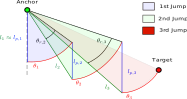
\includegraphics[width=\columnwidth]{figs/multiple_jumps_heuristics.pdf}
	\caption{Heuristics for multiple jumps}
	\label{fig:muti_jumps}
\end{figure}

\section{Reachability and Lyapunov}

Let us consider the system canonical form~\eqref{eq:CanonicalForm},
and let us consider that the inputs $F_{u,n}$, $F_{u,t}$ and $F_{r}$
are all fully available to control the system. By computing the
involutive distribution $\Delta_n$, if it is nonsingular the system is
locally reachable~\cite{isidori1985nonlinear}. As such, consider the
system state definition in~\eqref{eq:State}.


%%%%%%%%%%%%%%%%%%%%%%%%%%%%%%%%%%%%%%%%%%%%%%%%%%%%%%%%%%%%%%%%%%%%%%%%%%%%%%%%

% that's all folks

\bibliographystyle{IEEEtran}

\bibliography{include/biblio}


\end{document}